\chapter{Theoretische Grundlagen}
Dieses Kapitel erläutert die Grundlagen die zum 
Verständnis dieser Arbeit notwendig sind. 

%TEXT!!!!

\section{Docker}

In diesem Abschnitt wird die Technologie \glqq Docker\grqq{} näher erläutert und
nicht das Unternehmen \glqq Docker, Inc.\grqq{}, dass für die maßgebliche Entwicklung dessen verantwortlich ist.
Angefangen mit der Terminologie, zum deutlicheren Verständnis der nächsten Abschnitte.

\subsection{Terminologie}
\begin{itemize}
    \item \textbf{Container}: Isolierter Prozess mit einer laufenden Anwendung.
    \item \textbf{Volumes}: Persistente Daten eines Containers.
    \item \textbf{Image}: Einheit mit ausführbaren Code, Abhängigkeiten und Betriebssystem. Aufgeteilt in mehreren Schichten.
    \item \textbf{Dockerfile}: Datei zum erstellen von einem Docker Image.    
\end{itemize}

\subsection{Architektur}
Die Docker Technologie ist in der Programmiersprache "GO" geschrieben und nutzt Funktionalitäten des
Linux Kernels, wie cgroups und namespaces \cite{dockergetstarted}.
Namespaces ermöglichen die Isolation von Prozessen in sogenannte Container, welche unabhängig voneinander arbeiten.
Diese beeinhalten alle nötigen Abhängigkeiten zur Ausführung der vordefinierten Anwendung.
Container gewinnen dadurch an Portabilität, die ein bereitstellen auf Infrastrukturen mit der containerd
Laufzeit ermöglichen.
Die Laufzeit setzt sich aus \glqq runc\grqq{} einer low-Level Laufzeit und \glqq containerd\grqq{} einer higher-Level
Laufzeit zusammen (vgl. Abbildung~\ref{fig:dockerarch}).
Runc dient als Schnittstelle zum Betriebssystem und startet und stoppt Container.
Containerd verwaltet die Lebenszyklen eines Container, ziehen von Images, erstellen von Netzwerken und
Verwaltung von runc.
Die Allgemeine Aufgabe des Docker Daemons ist es eine vereinfachte Schnittstelle für die Abstraktion
der unterliegenden Schicht zu gewährleisten. Wie zum Beispiel dem verwalten von Images, Volumes und Netzwerken \cite{dockerdeep}.
Auf die Orchestrierung mit Swarm wird nicht weiter eingeganen, da sie zum Verständnis nicht nötig ist.


\begin{figure}
    \centering
    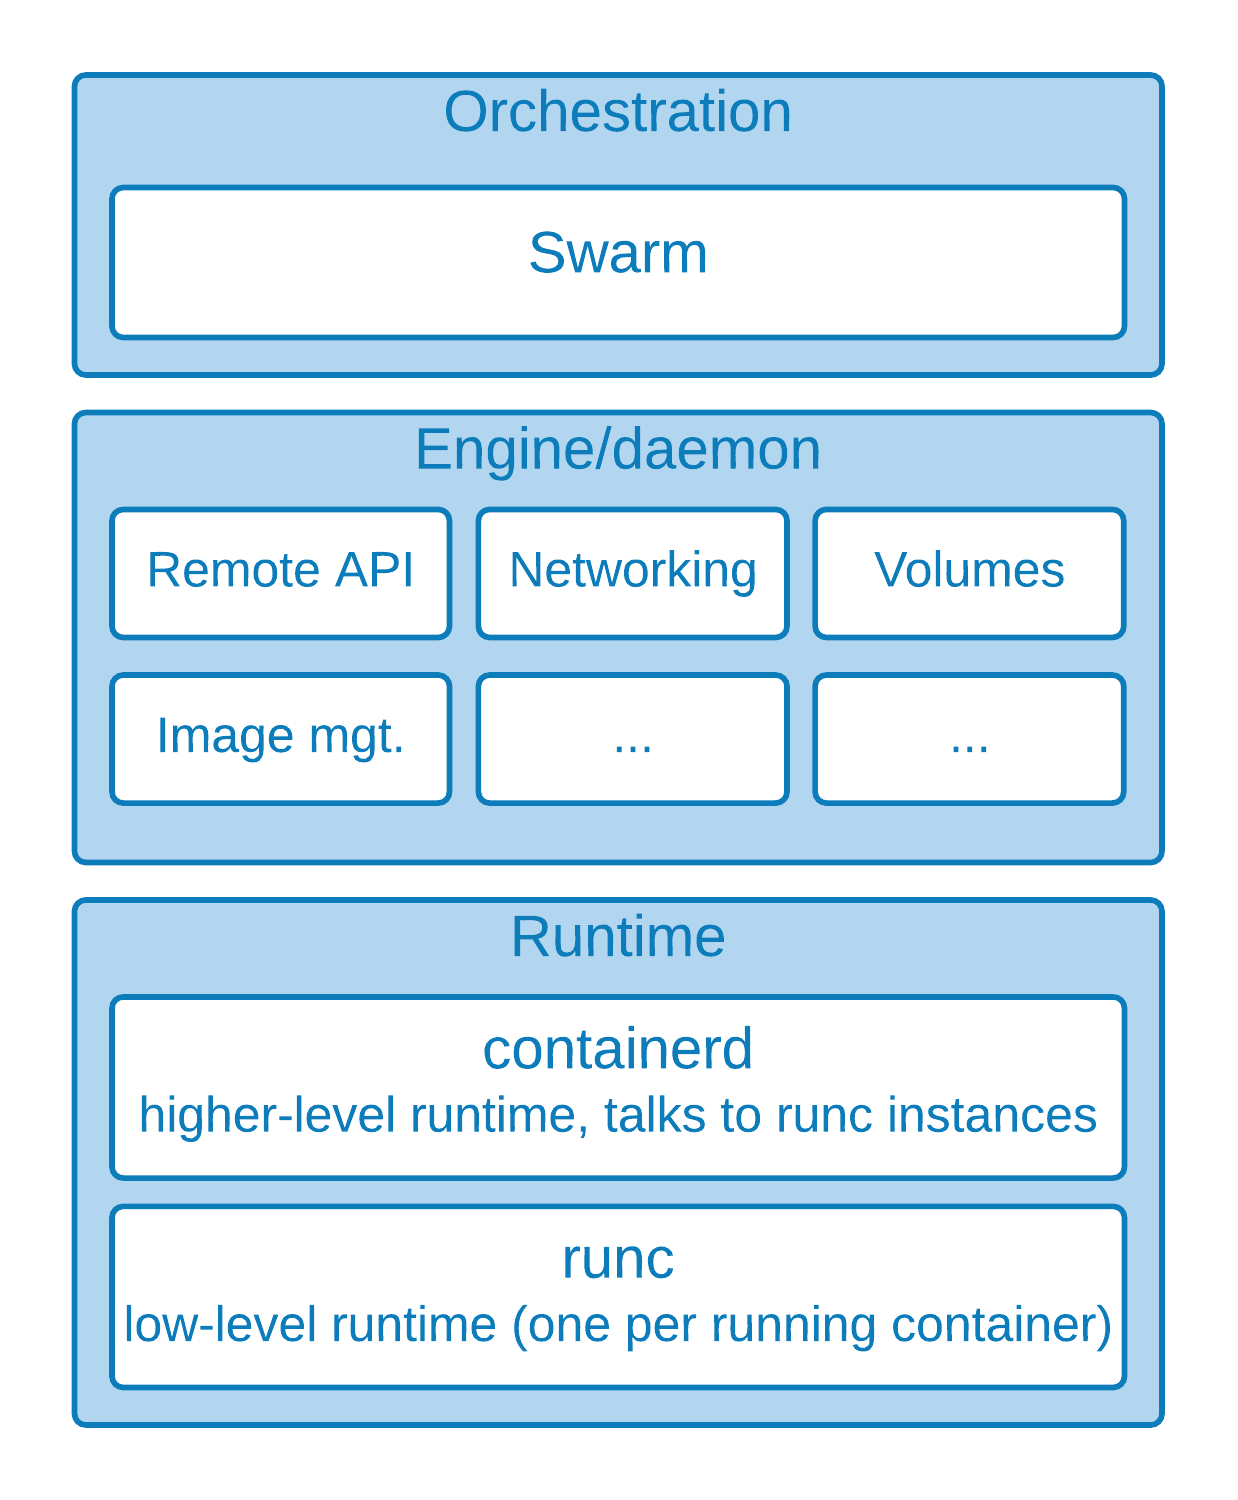
\includegraphics[width=0.5\columnwidth]{images/DockerArch.png}
    \caption{Docker Architektur \protect\cite{dockerdeep}}
    \label{fig:dockerarch}
\end{figure}

\section{Microservice}
\subsection{Aufbau}
\subsection{Entwicklung}
\subsection{Dezentrale Datenmanagement}


\section{Kubernetes}
\subsection{Architektur}
\subsection{Lightweight Kubernetes}
\subsection{Hybrid Cloud}
\subsection{Rancher}


%\subsubsection{Ein Unterabschnitt}
